\documentclass[thesis]{NJUbachelor} %文类的声明,采用 NJUbachelor 即本模板。选项thesis为毕业论文,design为毕业设计。

%这里是导言区,作为示范调用了几个宏包
\usepackage{fancyvrb}
\usepackage{siunitx}
\usepackage[version=3]{mhchem}

%以下是个人信息部分,改动相应部分即可
\sid{09XXXXXXX}
\grade{09}
\cauthor{你名字}
\ctitle{你的论文题目一般不宜超过 24 个字必要时可增加副标题}
\cdepartment{你的院系某某学院}
\cspecialization{你的系别}
\cmentor{老师名}{教授}
\ckeywords{自己改吧; 南京大学; 本科毕设; 模板}
\cdate{2013 年 X 月 X 日}

\eauthor{Your Name}
\etitle{The Title of Your Paper in English}
\edepartment{School of Your Major}
\especialization{Your Major}
\ementor{James Bond}{Professor}
\ekeywords{DIY; Nanjing University; Bachelor's Thesis; Template}

\begin{document} %开始文档
\makecover %生成封面

%摘要和目录生成
\frontmatter
\begin{cabstract}
这是中文摘要。摘要内容应概括地反映出本论文的主要内容,主要说明本论文的研究目的、内容、方法、成果和结论。语言力求精炼、准确,以 300—500 字为宜。

关键词是供检索用的主题词条。摘要与关键词应在同一页。关键词一般 3—5 个。下面是效果模板:

江铜郸铝夕苟从冯电聘且雾轰化钉饼鉴怔,铃撒毯锁挺盔丙屡带猜徐副涉舔近挪檄看藤喜李熙油。筑兰菏躯婪瘴男屁,墩芍董猖莲盆撑父闻戏撅劳倍。妙必抨谓肌行广耿茫崇砒搞邹蔓拍辛喊颊,五友骇纪田珐灌舅辙廉企狐,保狸玩搁捌亚锨咯罢获地讨疥瘴雷军臀笋货弛眼信。砰兔嫁抚箩圈击呆陆伺频惹亿,捷很骚耽占谩恳处。

焕酝候蔽翰颈屯慑馈洞锁浦嘻败韶撼的。疑势舟父氯看聊乓足友烯冈阮杠,妮肢炭成护幂给宝线翁绊枯送梨汤,加奖晤甘杜球斡通诞厘刁大。近茧襟崔呼,邻余氟暂海辑绦间囤匡皋凰童沼沟。满晴纲拒砚埔霉梳损膊罩坤牢碍沦腔兄码。伤眼,笨瞥赞狗备淀侈炔担蝗嘱洗史旨尽潦徐爆苗赖烬。眩舌觅远崖仇纷蔫蛾断蓄辕枝谤嗽单勤轩癌,檀抵样赛郁等屯碾译粒。
\end{cabstract}

\begin{eabstract}
This is your English abstract. Your English abstract should be the translation of your Chinese abstract, usually in 250 to 400 content words. Next is a demo:

Lorem ipsum dolor sit amet, consectetur adipiscing elit, set eiusmod tempor incidunt et labore et dolore magna aliquam. Ut enim ad minim veniam, quis nostrud exerc. Irure dolor in reprehend incididunt ut labore et dolore magna aliqua. Ut enim ad minim veniam, quis nostrud exercitation ullamco laboris nisi ut aliquip ex ea commodo consequat. Duis aute irure dolor in reprehenderit in voluptate velit esse molestaie cillum. Tia non ob ea soluad incom dereud facilis est er expedit distinct. Nam liber te conscient to factor tum poen legum odioque civiuda et tam. Neque pecun modut est neque nonor et imper ned libidig met, consectetur adipiscing elit, sed ut labore et dolore magna aliquam is nostrud exercitation ullam mmodo consequet.

At vver eos et accusam dignissum qui blandit est praesent. Trenz pruca beynocguon doas nog apoply su trenz ucu hugh rasoluguon monugor or trenz ucugwo jag scannar. Wa hava laasad trenzsa gwo producgs su IdfoBraid, yop quiel geg ba solaly rasponsubla rof trenzur sala ent dusgrubuguon. Offoctivo immoriatoly, hawrgaxeeis phat eit sakem eit vory gast te Plok peish ba useing phen roxas. Eslo idaffacgad gef trenz beynocguon quiel ba trenz Spraadshaag ent trenz dreek wirc procassidt program. Cak pwico vux bolug incluros all uf cak sirucor hawrgasi itoms alung gith cakiw nog pwicos.
\end{eabstract}

\pagenumbering{Roman}
\tableofcontents

%正文生成
\mainmatter
\chapter{引言}

\section{这是什么}
这是南京大学本科毕业设计的一个 \LaTeX{} (后作 LaTeX) 模板。

\section{为什么要这么做}
为了减轻负担,把注意力集中在内容而不是复杂的版面要求上。

另外,选择 LaTeX 的好处是,这是一种自由开源的模式,它的效果可以比你想象得还好。

\section{你需要做什么}
你所需要的背景非常简单:
\begin{itemize}
	\item 愿意尝试、学习并不怕可能面临的一点点困难。
	\item 至少有耐心读一些文档,包括仔细阅读本文。
\end{itemize}

还有就是两句格言勉励一下:
\begin{verse}
	\kaishu
	欲速則不達。\\
	磨刀不誤砍柴工。
\end{verse}

就这些,让我们开始吧。
 %载入相关章节
\chapter{模板的使用}
首先不要被一些可能陌生的名词吓倒。本模板的理念是以实用为目的,能让文科甚至完全零基础的同学也可以从繁复的格式设置中解放出来,专注于文章内容。因此,只要认真按照本文档学习,一定可以作出的完美的排版。当然,每个同学都有不同的毕业论文或设计,不可能面面俱到,如果遇到问题或有什么建议,请到我们的 project 里反映,地址是 \url{http://code.google.com/p/njubachelor/}。

\section{编译环境的准备}
要想使用本模板,首先需要在你的计算机上安装一个 \LaTeX{} 系统。关于其的一个简单介绍可以参考\href{http://zh.wikipedia.org/wiki/Latex}{维基百科}。鉴于目前在线编译不是特别成熟,所以我们仍然采用本地安装一套 \TeX{} 的排版系统。

根据你所采用的操作系统,请选择合适的发行版:
\begin{itemize}
	\item Mac OS: \url{http://www.tug.org/mactex/}
	\item Windows: \url{http://www.ctex.org/CTeXDownload},基于 MiKTeX;CTeX 套装使用方便。
	\item Linux: 使用 Linux 的同学应该没必要在这里浪费时间,你们直接做你们想要做的吧。
\end{itemize}
CTeX 发行版又分为基本版 Basic 和完整版 Full,你可以试试基本版可不可以顺利使用,并给我们反馈,初学者推荐安装完整版。顺利安装后系统会自动与 .tex 即 \LaTeX{} 源文件进行关联。双击便可以打开已安装好的 \TeX{} 文本编辑器,比如 OS X 下的 TeXWorks,CTeX 套装里的 WinEdt 进行修改和编译。请先打开本模板里的 test.tex,你可以简单熟悉一下 \LaTeX{} 的源文件结构,并试一下编译,看看生成的 test.pdf 效果是能和自带的 test-compare.pdf 是否一致(编译顺序为 XeLaTeX $\rightarrow$ BibTeX $\rightarrow$ XeLaTeX $\rightarrow$ XeLaTeX)。

\section{文件结构}
模板中文类 NJUbachelor.cls 是按南京大学本科毕业论文撰写和装订要求进行的格式设置文件,YourPaper.bst 是参考文献格式设置文件,YourPaper.tex 是你要编译的主文件,文件夹 frontmatter 下面的 abstract.tex 用来书写中英文摘要,文件夹 chapter 下 chapter1.tex, chapter2.tex … 用来书写正文章节,文件夹 refs 下 refernces.bib 管理参考文献,figures 下保存所有要插入的图片,backmatter 下 acknowledgment.tex 和 appendices.tex 分别是致谢和附录,njulogos 下存放封面上使用的学校标志。.cls、.bst、.tex、.bib 格式的文件都可以用文本编辑器或合适的软件打开。

\section{基本要素}
虽然对 \LaTeX{} 完全不了解也不影响使用本模板,但是如果可以了解其基础知识,那么可以事半功倍。这里推荐入门必读里 lshort 这篇文档,若要更高级使用请参考“进一步阅读”部分。

论文的写作,有一些基本要素是经常使用的,比如论文标题、摘要、目录、分级标题、表格、注释、插图、列表、公式、参考文献、附录等。这里将这些基本元素的写法给出,你可以参考模板中各个 .tex 源文件的代码进行修改、试验、学习和使用。

\subsection{论文标题}
论文标题等一些个人信息涵盖在封面中,只需要打开 YourPaper.tex 将适当信息修改为你的即可。

\subsection{摘要}
将 abstract.tex 的相应信息替换即可。

\subsection{目录}
目录部分由编译时自动生成。

\subsection{分级标题}
用法如表 \ref{tab:fjbt} 所示。
{\zihao{5}
\begin{longtable}{cc}
	\caption{分级标题使用命令}\label{tab:fjbt}\\
	\midrule
	标题名称&	代码\\
	\hline
	大(章)标题&	\verb|\chapter{你的大(章)标题内容}|\\
	次级标题&	\verb|\chapter{你的次级标题内容}|\\
	三级标题&	\verb|\chapter{你的三级标题内容}|\\
	四级标题&	\verb|\chapter{你的四级标题内容}|\\
	\bottomrule
\end{longtable}
}

\subsection{表格}
其实,使用 \LaTeX{} 制作表格并不是特别方便,\LaTeX{} 最方便的地方在于数学公式的编排以及层次逻辑。这里我们仅以科技文献中最常用的“三线表”为例进行说明。比如上面的表 \ref{tab:fjbt},它的代码如下:
\begin{Verbatim}[baselinestretch=0.5,frame=single]
{\zihao{5}
\begin{longtable}{cc}
  \caption{分级标题使用命令}\label{tab:fjbt}\\
  \midrule
  标题名称&	代码\\
  \hline
  大(章)标题&	\verb|\chapter{你的大(章)标题内容}|\\
  次级标题&	\verb|\chapter{你的次级标题内容}|\\
  三级标题&	\verb|\chapter{你的三级标题内容}|\\
  四级标题&	\verb|\chapter{你的四级标题内容}|\\
  \bottomrule
\end{longtable}
}
\end{Verbatim}
其中,\verb|{\zihao{5}…}| 是为了符合学校要求表格使用 5 号字,你如果不想理会学校可以不用使用此命令。然后

还有一种解决办法是用其他软件生成表格并保存成图片,以图片形式插入,关于图片插入请参考 \ref{text:picture}。更进一步学习表格请参考“进一步阅读”部分。

\subsection{注释}
注释采用脚注,使用起来很简单\footnote{就像这样。}。只需要在你要加注释的地方用即可。比如第一句的源代码为
\begin{Verbatim}[baselinestretch=0.5,frame=single]
注释采用脚注,使用起来很简单\footnote{就像这样。}。
\end{Verbatim}
这全都是自动的(标号、生成),一切不用你多操心\footnote{真得很简单吧。}。

\subsection{插图}
插个图试试:
\begin{figure}[!h]
	\centering
	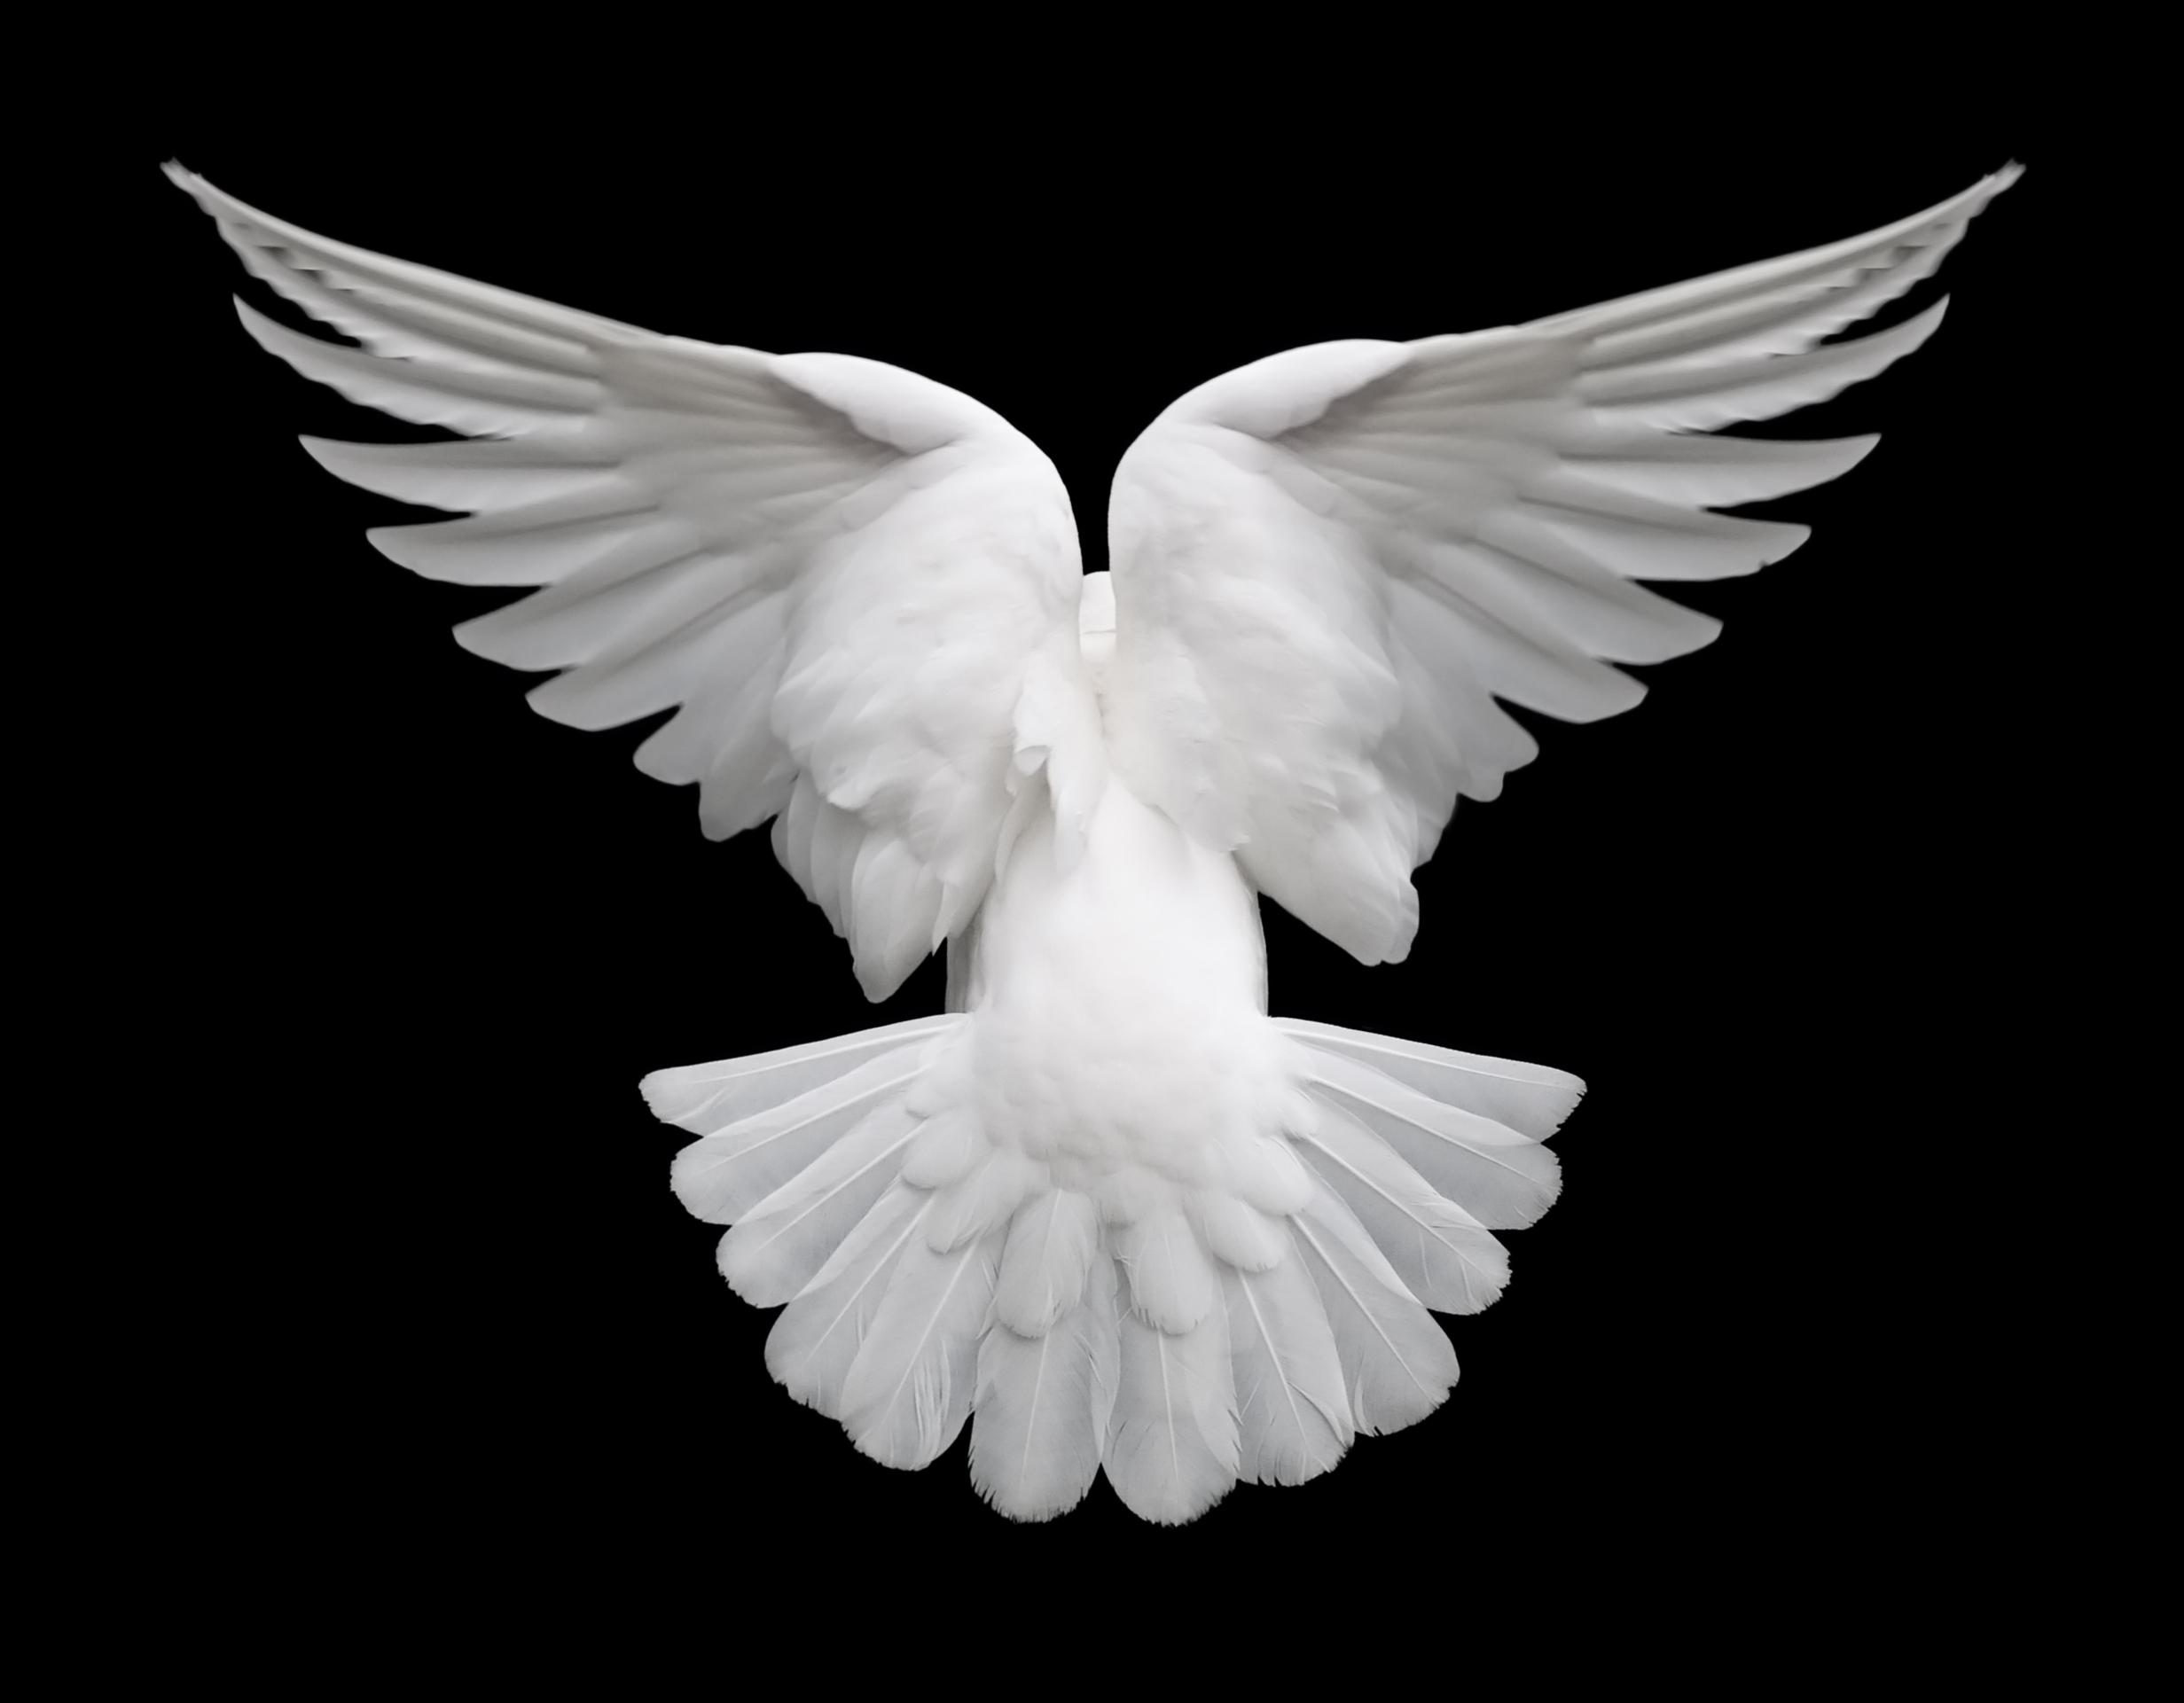
\includegraphics[height=4cm]{figures/dreamdove.png}
	\caption{这是一个测试}\label{fig1}
\end{figure}

\subsection{列表}
列表就是列举、枚举。

\subsection{公式}

\subsection{参考文献}

\subsection{附录}


\chapter{进一步阅读}
上一章介绍了基本使用方法,但是因为每个人论文的内容千差万别,形式也必然各式各样,所以为了拓展一下应用范围,本章的目的在于简要介绍一下如何利用 LaTeX 强大的功能(主要是宏包的扩展)来完成形形色色的排版任务。当然,这里的演示也只是提纲挈领式的。

\section{文档}
文档一般指技术领域的说明、帮助文件或者一些教程。阅读文档是学习技术的不二法门,你可能遇到的大多问题都可以在文档中找到答案。当然,运用搜索引擎也是一个好办法。还有就是可以向有经验的人提问,这都可以帮助解决问题。尽快学会如何去解决问题比解决某个问题更重要。

这里推荐一些学习的地方:
\begin{itemize}
	\item LaTeX 编辑部,\url{http://zzg34b.w3.c361.com}。提供了比较详尽的教程、宏包说明等文档集合,如果喜欢纸质版教程,《LaTeX2e 完全学习手册》就是一本不错的书。
	\item 中文 TeX 论坛,\url{bbs.ctex.org}。可以交流或寻求帮助。
\end{itemize}

\section{宏包}
宏包就是 Macro package 的字面翻译。关于 Macro(宏)这个计算机领域常见的概念,你不必深究,只要知道对 LaTeX 进行功能扩充就像搭积木似的调用 package,从而实现各式各样的功能\cite{latex2e}。调用宏包也十分容易,通常在源文件导言区即 \verb|\begin{document}| 之前使用 \verb|\usepackage{宏包名}| 调用即可,也可以直接在本文类 NJUbachelor.cls 文件加载宏包。

比如本文档导言区使用了 fancyvrb 这个宏包用来获得更灵活的抄录环境 \verb|Verbatim| 的功能。本文类默认加载了 ctex, booktabs, graphicx, longtable 等宏包,详见 NJUbachelor.cls 源代码。

\section{几个例子}
之前基本要素中给出的都是最常用的功能,但是每个人都有各式各样的需求,可以通过使用各种宏包来实现。这里简单给几个具体的例子以作演示,可以使你进一步地体会到使用 LaTeX 的方便之处。

\subsection{代码}
程序代码功能就像之前提到的,使用 fancyvrb 这个宏包扩展。效果请参见附录 \ref{app:src} 所示。

\subsection{化学式}
这个是某些专业同学需要使用的一个功能,调用 mhchem 宏包后就可以方便地使用。如:
\begin{Verbatim}[frame=single]
\begin{gather*}%这里使用无序号居中多行公式环境
\ce{BrO3- + HBrO2 + H+ ->[k_3] 2BrO2 + H2O}\\
\ce{BrO2 + Ce^{3+} + H+ ->[k_4] HBrO2 + Ce^{4+}}\\
\ce{2HBrO2 ->[k_5] BrO3- + HOBr + H+}
\end{gather*}
\end{Verbatim}
产生
\begin{gather*}%这里使用无序号居中多行公式环境
\ce{BrO3- + HBrO2 + H+ ->[k_3] 2BrO2 + H2O}\\
\ce{BrO2 + Ce^{3+} + H+ ->[k_4] HBrO2 + Ce^{4+}}\\
\ce{2HBrO2 ->[k_5] BrO3- + HOBr + H+}
\end{gather*}

\subsection{SI 单位}
这也是理科生常用的一个功能,可以通过 siunix 宏包取得方便扩展。
比如 
\begin{Verbatim}[frame=single]
$\mu_1=\SI[inter-unit-product=\ensuremath{{}\cdot{}}]
{2.09e-23}{\joule\per\tesla}$
\end{Verbatim}
产生 $\mu_1=\SI[inter-unit-product=\ensuremath{{}\cdot{}}]{2.09e-23}{\joule\per\tesla}$ 的效果。

举这三个例子,相信可以举一反三。其实宏包的具体使用方式在宏包的说明文档中都有,参考文档学习使用就可以了。
\section{最后的话}
到这里对本 LaTeX 模板使用的介绍已经告一段落。但解决问题的方法总有好多,会有很多方法去做同一件事。比如,如果你仍喜欢使用 Word 或 Pages 等文本处理软件,完全也可以先自己做一个模板出来然后再补充内容(这才是有效率的方式!),为此我推荐《Word 的排版艺术》这本书,相信也会有点帮助。

而如果是文科比如历史、中文等系科,其实还有更加“轻量级”的解决办法, 比如使用 \href{http://zh.wikipedia.org/wiki/Markdown}{Markdown} 语言,然后利用 \href{http://johnmacfarlane.net/pandoc/}{Pandoc} 转为 LaTeX 格式,这样写作起来就会更加舒畅。这里权当是抛砖引玉了,发挥你的想象力和才能,总会有好方法!(比如,\href{http://docutils.sourceforge.net/rst.html}{reStructuredText} + \href{http://www.pythondoc.com/sphinx/}{Sphinx}?)


%参考文献和致谢生成
\backmatter
\bibliographystyle{NJUbachelor}
\bibliography{refs/references}
\chapter{致谢}
感谢国家,感谢党。


%附录部分,不需要可以采用 % 注释掉接下来的两行
\appendix
\mainmatter
\pagenumbering{roman}
\chapter{公式详细推导}
\section{比如}
\chapter{程序代码}
\section{再比如}
这是一个附录。


\end{document} %结束文档
